% =============================================================================
% 4.2 基于代码生成的确定性统计分析
% 草稿版本：v0.2 (2026-05-05)
%   v0.1：完成正文初稿。
%   v0.2：嵌入 1 张图与 3 张表，由对应 \reffig / \reftab 引用就近浮动。
% 字数：约 2000 字（不含图表 caption）
% 风格规则：v0.2 风格（无 \textbf / \textit / 引例括号 / 双引号 / 破折号）
% 引用：\cite{ref10, ref20, ref21, ref22, ref23, ref29}
% 图表：
%   - 图 \reffig{fig:code-gen-flow}       代码生成与受限沙箱执行流程图
%   - 表 \reftab{tab:code-bench-design}   18 条评测集任务分布
%   - 表 \reftab{tab:code-eval-overall}   3 档消融总表
%   - 表 \reftab{tab:code-eval-category}  按用例类别拆分
% 依赖宏包：booktabs / tabularx / graphicx（主稿已加载）
% =============================================================================

\subsection{基于代码生成的确定性统计分析}
\label{sec:code-execution}

前节通过双通路 RAG 解决了数值到语义标签的离散映射问题。然而气象任务
还涉及大量统计计算性需求，例如过去一周武汉最高温的平均值是多少、过去
14 天里有几天下了雨、降水量前三名的日期分别是哪几天。这类任务的输出
是一个数值或序列。如果继续让大语言模型自由发挥，会触发与上节分级幻觉
本质不同的另一类幻觉，即数值计算幻觉。Hong 等 \cite{ref20} 在 Data Interpreter 中指出，让
大语言模型直接进行数值聚合相当于让它在没有草稿纸的情况下心算，工作记忆
容量限制下错误率显著高于把任务转化为可执行代码。本节据此设计了基于
代码生成与受限沙箱执行的确定性统计分析方案，并通过对照实验量化了与
大语言模型自由直算之间的准确率差距。

\subsubsection*{4.2.1 \quad 代码生成器与受限沙箱的协同设计}

整个分析管线由三个组件协同完成，整体流程如 \reffig{fig:code-gen-flow}
所示。

\begin{figure}[H]
    \centering
    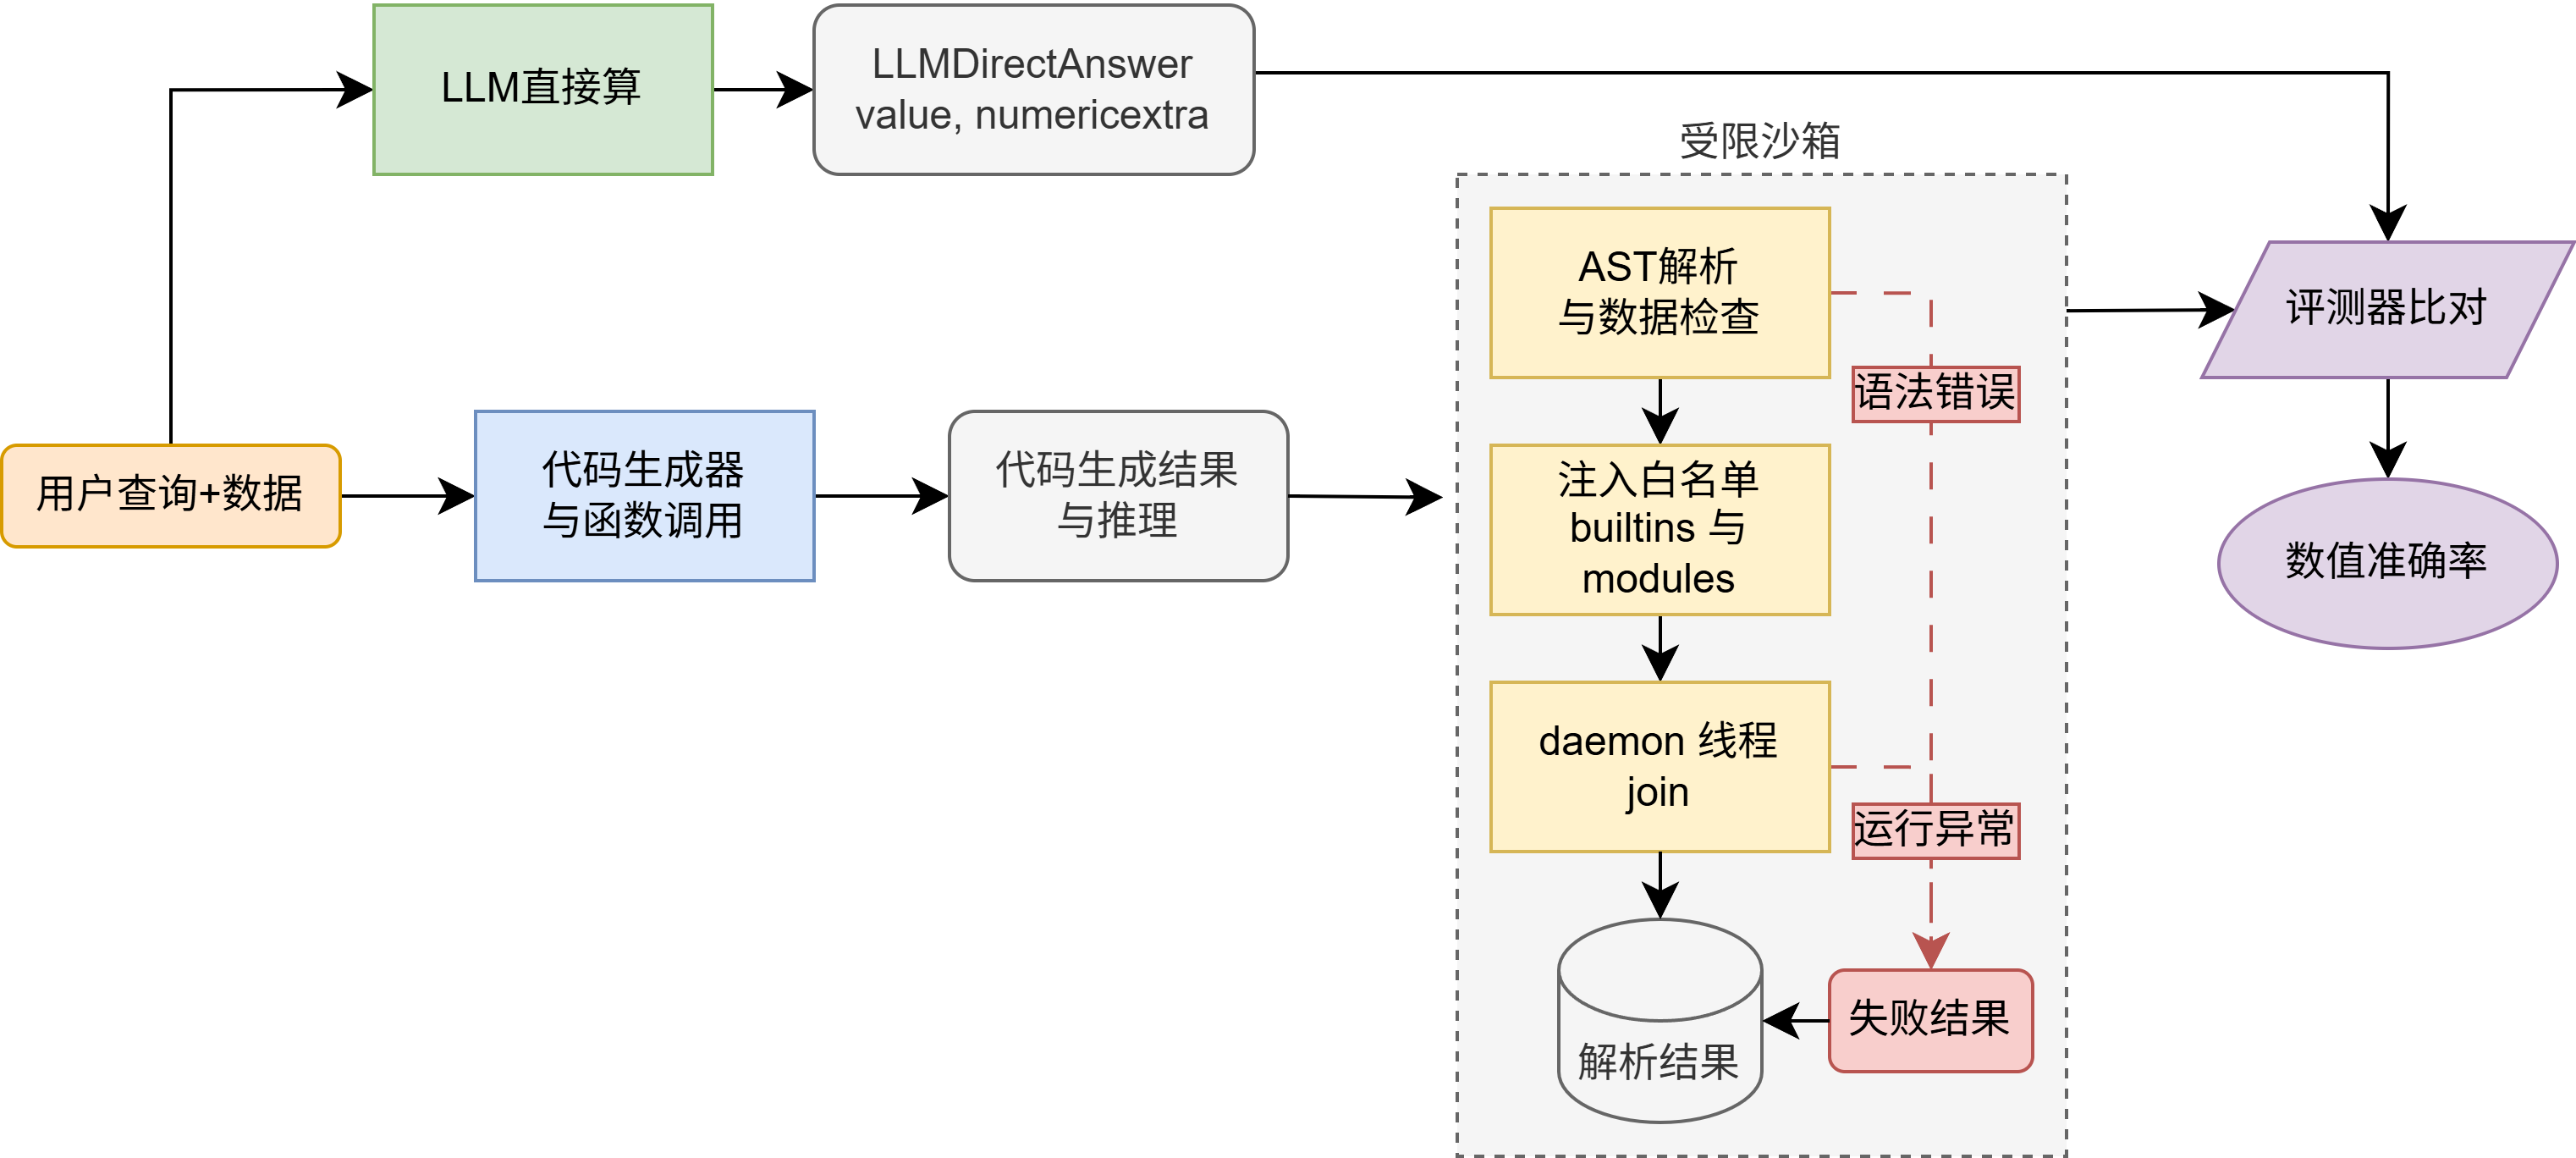
\includegraphics[width=\linewidth,height=0.4\textheight,keepaspectratio]{figures/code-gen-flow}
    \caption{代码生成与受限沙箱执行流程图}
    \label{fig:code-gen-flow}
\end{figure}

第一是位于 \texttt{src/\bk{}analysis/\bk{}code\_\bk{}generator.\bk{}py} 的代码生成器，
通过 OpenAI 兼容协议下的 function calling 模式让大语言模型输出结构化
\texttt{CodeGenResult} 对象，包含 \texttt{code} 与 \texttt{reasoning}
两个字段。Prompt 中显式约定生成代码必须定义顶层函数 \texttt{compute(data)}，
\texttt{data} 由调用方注入，函数返回值即最终答案。第二是位于
\texttt{src/\bk{}tools/\bk{}code\_\bk{}executor.\bk{}py} 的受限沙箱，对生成代码做隔离执行。
第三是上层评测脚本，把代码生成器的输出送入沙箱执行并比对期望值。

受限沙箱的设计借鉴了 Schick 等 \cite{ref21} 在 Toolformer 中关于工具
调用安全边界的论述，但裁剪到本文场景下的最小可用形态，包含四项约束。
其一是显式 builtins 白名单。沙箱仅暴露 \texttt{abs}、\texttt{sum}、
\texttt{max}、\texttt{min}、\texttt{round}、\texttt{sorted}、
\texttt{enumerate}、\texttt{iter}、\texttt{next} 等数据处理类内置函数，
对 \texttt{open}、\texttt{eval}、\texttt{exec}、\texttt{compile}、
\texttt{\_\bk{}\_\bk{}import\_\bk{}\_\bk{}} 等高危内置实施显式黑名单。其二是模块白名单。
沙箱将 \texttt{math} 与 \texttt{statistics} 两个只读数学库注入受限
全局命名空间，禁止生成代码通过 \texttt{import} 引入任何其他模块。
其三是墙钟超时。每次调用 \texttt{compute(data)} 在 daemon 线程内执行，
通过 \texttt{Thread.\bk{}join(timeout)} 实现 5 秒墙钟超时，避免生成代码中
意外死循环阻塞主流程。其四是结构化错误捕获。语法错误、缺函数、运行时
异常与超时四类失败模式统一封装在 \texttt{ExecutionResult} 对象中返回，
不会以异常形式污染上游评测脚本。

需要明确的是，本文设计的沙箱属于轻量原型，主动放弃了完整的安全隔离。
真实生产环境下应当使用 RestrictedPython、Pyodide 或 Docker 容器实现
进程级隔离 \cite{ref23}。本文限定在毕业设计研究范围内，沙箱的核心
目标是为代码生成可靠性的可重复测量提供执行通道，而非抵御主动恶意攻击。
完整的安全沙箱方案在 \ref{sec:future-work} 节作为未来工作展开。

\subsubsection*{4.2.2 \quad 三档消融实验设计与核心结果}

为量化代码生成与执行带来的准确率提升，本文构建了 18 条覆盖六类统计模式
的评测集 \texttt{code\_\bk{}exec\_\bk{}bench.\bk{}jsonl}，详见
\reftab{tab:code-bench-design}。六类模式分别对应平均、极值、求和、差值、
计数、排序，每类用例都故意包含若干边界情形，例如平均值类中含 24.95 的
银行家舍入边界、计数类中含 35.0 的高温阈值平等、求和类中含条件求和。
每条用例标注期望值与容差，并按答案结构分为标量、日期、日期加数值复合、
时刻加数值复合、有序列表共五种期望类型。

\begin{table}[!htbp]
    \centering
    \caption{代码执行评测集任务分布（6 类统计模式，共 18 条用例）}
    \label{tab:code-bench-design}
    \song\wuhao
    \begin{tabular}{lrll}
        \toprule
        类别 & 用例数 & 期望答案类型 & 设计要点 \\
        \midrule
        平均 average & 5 & scalar & 含整除、近似与银行家舍入边界 24.95 \\
        极值 extreme & 3 & date / time + value & 同时返回日期或时刻与对应数值 \\
        求和 sum & 2 & scalar & 7 天累计与高温日条件求和 \\
        差值 diff & 4 & scalar 或 date + value & 日较差最大、跨日极差、同比差 \\
        计数 count & 2 & scalar & 含 35.0 °C 高温阈值平等 \\
        排序 sort & 2 & ordered\_list / date & Top-$K$ 排序与第二高温日期 \\
        \midrule
        \multicolumn{1}{c}{合计} & 18 & --- & --- \\
        \bottomrule
    \end{tabular}
\end{table}

实验设计三档消融以隔离不同来源的能力贡献。\texttt{oracle} 档直接读取
期望值，作为评测器自校验天花板，验证比较函数本身的正确性。
\texttt{llm\_\bk{}direct} 档让大语言模型同时看到 query 与 data，但 prompt
明确禁止生成代码，要求其直接给出数值答案，作为大语言模型自由发挥的
对照。\texttt{llm\_\bk{}with\_\bk{}code} 档让大语言模型生成 \texttt{compute(data)}
代码并送入受限沙箱执行，取沙箱返回值作为最终答案。三档使用同一被测
模型 GLM-5.1，避免引入模型差异。

核心结果见 \reftab{tab:code-eval-overall}。\texttt{oracle} 档准确率
100.0\%，证明评测器自身没有偏差。\texttt{llm\_\bk{}direct} 档数值准确率
仅为 66.7\%，\texttt{llm\_\bk{}with\_\bk{}code} 档数值准确率提升至 88.9\%，
两档之间存在 22.2 个百分点的差距。代码生成率与代码可执行率均为 94.4\%，
表明大语言模型在 function calling 模式下生成可执行代码的能力是稳定的，
失败主要来自单条用例上的算法错误而非工具调用失败。

\begin{table}[!htbp]
    \centering
    \caption{代码执行三档消融总表（18 条评测集）}
    \label{tab:code-eval-overall}
    \song\wuhao
    \begin{tabular}{lccc}
        \toprule
        指标 & oracle & llm\_direct & llm\_with\_code \\
        \midrule
        数值准确率 & 100.0\% & 66.7\% & 88.9\% \\
        代码生成率 & --- & --- & 94.4\% \\
        代码可执行率 & --- & --- & 94.4\% \\
        \bottomrule
    \end{tabular}
\end{table}

按用例类别拆分后差距进一步放大，详见 \reftab{tab:code-eval-category}。
极值类用例上 \texttt{llm\_\bk{}direct} 准确率为 0.0\%，\texttt{llm\_\bk{}with\_\bk{}code}
为 66.7\%，差距 66.7 个百分点。计数类用例上 \texttt{llm\_\bk{}direct} 为
50.0\%，\texttt{llm\_\bk{}with\_\bk{}code} 为 100\%，差距 50 个百分点。求和与
排序两类则两档持平在 100\%。这一分布揭示了一条规律：大语言模型在简单
累加与天然排序任务上能够依靠语料能力做对，但只要任务需要伴随状态维护
或离散计数，例如在找最大值的同时记录对应日期，就会犯错。这与认知科学
中关于工作记忆容量限制的发现一致。代码执行的本质是给大语言模型配上一支
笔与一张草稿纸，把心算换成笔算 \cite{ref20, ref29}。

\begin{table}[!htbp]
    \centering
    \caption{代码执行评测按用例类别拆分（数值准确率）}
    \label{tab:code-eval-category}
    \song\wuhao
    \begin{tabular}{lrccc}
        \toprule
        类别 & 用例数 & llm\_direct & llm\_with\_code & 差距 \\
        \midrule
        极值 extreme & 3 & 0.0\% & 66.7\% & $+66.7$ pp \\
        计数 count & 2 & 50.0\% & 100.0\% & $+50.0$ pp \\
        平均 average & 5 & 80.0\% & 100.0\% & $+20.0$ pp \\
        求和 sum & 2 & 100.0\% & 100.0\% & 持平 \\
        排序 sort & 2 & 100.0\% & 100.0\% & 持平 \\
        差值 diff & 4 & 75.0\% & 75.0\% & 持平（命名漂移） \\
        \bottomrule
    \end{tabular}
\end{table}

\subsubsection*{4.2.3 \quad 大语言模型直算的四类典型幻觉模式}

通过对 \texttt{llm\_\bk{}direct} 档 6 条失败用例的逐条分析，本文归纳出大
语言模型在数值任务上的四类典型幻觉模式，每类都构成代码执行不可替代
的具体证据。

第一类是数数错误，对应用例 \texttt{count\_\bk{}001\_\bk{}rainy\_\bk{}days}。该用例
要求统计 14 天中降水量大于 0 的天数，正确答案为 7。大语言模型在
\texttt{reasoning} 字段中正确列举出了 7 个日期 04-02、04-03、04-05、
04-08、04-09、04-12、04-14，但 \texttt{value} 字段却给出了 6。这种
推理过程与最终答案自相矛盾的幻觉是最危险的形式，用户阅读 reasoning
通常会被说服，难以察觉数值错误。

第二类是舍入不一致，对应用例 \texttt{avg\_\bk{}005\_\bk{}feels\_\bk{}like}。8 小时
体感温度均值精确计算结果为 24.95，使用 Python \texttt{round} 的银行家
舍入向偶数舍入应得 24.9。大语言模型给出的答案是 25.0，并在 reasoning
中说明 24.95 保留 1 位小数为 25.0，反映其默认采用中学教科书的四舍五入
规则。这种语境敏感的精度幻觉在工程数据处理中是不可接受的，因为下游
所有数值处理都默认使用 Python 标准舍入。

第三类是 schema 不稳定，对应 \texttt{extreme\_\bk{}001} 至
\texttt{extreme\_\bk{}003} 与 \texttt{diff\_\bk{}001\_\bk{}max\_\bk{}diurnal} 共 4 条用例。
这些用例要求同时给出哪一天与对应数值，例如返回字典
\texttt{\{date: 2025-07-03, tempMax: 36.8\}}。Prompt 中已经明确要求
把日期放在 \texttt{value} 字段、把数值放在 \texttt{numeric\_\bk{}extra}
字段，但大语言模型在 function calling 下仍只填写日期字段，把数值留
作自由文本。Schema 的可靠性随复杂度上升急剧下降是大语言模型应用工程
中的经典痛点 \cite{ref22}。

第四类是字段命名漂移，仅出现在 \texttt{llm\_\bk{}with\_\bk{}code} 档的
\texttt{diff\_\bk{}001} 用例中。生成代码逻辑完全正确，找出了温差最大的
2025-09-18 一天，温差 22.7 摄氏度，但返回字典字段名为 \texttt{range}
而非期望的 \texttt{tempDiff}。这一失败模式与前三类性质不同，反映了
大语言模型在数据建模时命名约定不严格，可以通过更严格的 schema 约束
或下游适配层缓解。

将 4.1 与 4.2 两节合并观察，本文已经在分级 ID 编造、权威标准引用、
数值统计计算三个维度上量化了大语言模型自由发挥的不可靠性，并分别用
混合检索、确定性分级器、代码生成与受限沙箱执行三类机制构成了完整的
工具学习与计算辅助闭环。下一节将进一步讨论如何把这些机制的输出整合为
面向用户的自适应气象决策报告。

